\subsubsection{Factorization Based Sparse Solvers and Preconditioners for Exascale} \label{subsubsect:strumpack}

\paragraph{Overview} 
% \textit{Provide an overview of your project.  You might find that the introductory text from your Fall 2017 Project Summary \url{https://confluence.exascaleproject.org/display/1ST/Fall+2017+ECP+ST+Project+Summaries} useful as a starting draft.}
In this project we will deliver factorization based sparse solvers
encompassing the two widely used algorithm variants: supernodal
(SuperLU library) and multifrontal (STRUMPACK library). STRUMPACK is
further enhanced with scalable preconditioning functionality using
hierarchical matrix algebra. Both libraries are purely algebraic,
applicable to a large variety of application domains. We will address
several challenges that arise in Exascale computing, with the following
focus areas: 
(1) Develop novel approximation algorithms that have lower
arithmetic and communication complexity with respect to the input
problem size;
(2) Develop new parallelization strategies that reduce
inter-process communication and expose task parallelism and vectorization
for irregular computations involving sparse data structures to better
use on-node resources;
(3) Integrate our software into the higher level
algebraic solvers such as hypre, PETSc, Trilinos, and collaborate with
ECP application teams for application-specific and hardware-specific tuning
of the parameters space to achieve optimal efficiency of our solvers.

Our solver technology is essential for ECP, because many DOE simulation
and data analysis codes expected to run on the Exascale machines need
solutions of sparse algebraic systems, and many high fidelity simulations
involve large-scale multiphysics and multiscale modeling problems that
generate highly ill-conditioned and indefinite algebraic equations,
for which pure iterative methods such as Krylov and multigrid, albeit
readily parallelizable on large machines, cannot converge to the solution.
The factorization based algorithms being developed in our ECP project
represent an important class of methods that are indispensable building
blocks for solving those numerically challenging problems. Our software
can often be used as a reliable standalone solver, or as a preconditioner
for Krylov iterative methods, or as a coarse grid solver in multigrid
methods, just to name a few.


\paragraph{Key Challenges}
%\textit{Describe what is hard to do, why it is challenging.}
At Exascale we need to address several major challenges:
decreasing amount of memory per core, larger impact of communication
cost and load imbalance, more heterogeneous memory organization.
Our new design of algorithms and codes need to focus on
reducing communication and synchronization and task scheduling 
instead of floating point operation throughput. In sparse factorization
methods, we expect new bottlenecks in parts of the code
that previously received little attention. For example, the preprocessing
step involves numerical pivoting for selecting stable pivots and
symbolic factorization, which do not yet parallelize well on manycore
architectures with fine-grained parallelism.
At Exascale, direct solvers are more likely to
be used in a preconditioning strategy, for example, in block Jacobi
preconditioning, in domain decomposition methods or as coarse-grid
solvers in algebraic multigrid, which requires repeated triangular
solves. The challenge here is to mitigate the low arithmetic intensity
and high degree of data dependency.

Compared to iterative methods, the primary bottleneck of direct solvers
is the asymptotically higher growth in memory need and floating point
operations, especially for problems from three-dimensional geometry.
It is imperative to develop novel factorization methods which require
much less memory footprint and data movement.


\paragraph{Solution Strategy}
%\textit{Describe your basic strategy for addressing the challenges.}
We will address these challenges in several thrust areas.
The new techniques will be implemented in the two software packages SuperLU
and STRUMPACK. The former is a widely used sparse direct solver based on
supernodal factorization and the latter is a newer direct
solver/preconditioner package based on multifrontal factorization 
and hierarchical low-rank matrix structures.
% Parallel pre-pivoting for both packages.

The improvements for SuperLU will be mainly in two areas: (1) develop
a communication-avoiding 3D factorization code that have provably 
lower communication complexity; (2) develop a synchronization-avoiding
triangular solve code to enable more overlap of communications of different
processes at different substitution steps.

In addition to exploiting structural sparsity as SuperLU does, STRUMPACK
also exploits data sparseness in the dense blocks of sparse factors using
low-rank representations, which leads to linear scaling $O(n)$ or $O(n \log n)$
memory and arithmetic complexity for PDEs with smooth kernels.
The developments for STRUMPACK will focus several areas:
(1) develop robust stopping criteria --- both absolute and relative --- for
    adaptive (incremental) randomized sampling scheme to reveal numerical
    ranks in the low-rank compression routine. The goal is to use
    enough samples for stability, but not too many for efficiency;
(2) add OpenMP support for both HSS compression and ULV factorization routines,
    especially use OpenMP task construct to support irregular parallelism.
(3) reduce MPI communication in all stages of the code, including HSS
    construction, ULV factorization and triangular solve;
(4) in addition to HSS, develop codes to support other simpler low-rank
    format, such as HOLDR. The HSS format has asymptotically lower complexity
    than HOLDR, but has larger prefactor constant. We expect HSS to be more
    useful for large-scale problems while HOLDR is more useful for mid-range
    problems;
(5) work with the ECP application teams to examine their specific problem
    characteristics and develop the best clustering/ordering methods to 
    reveal low-rank structures.

\paragraph{Recent Progress}
%\textit{Describe what you have done recently.  It would be good to have some kind of figure or diagram in this section.}
We have made significant progress in the following areas:
\begin{enumerate}
\item We developed and evaluated a fully algebraic sparse preconditioner in 
      STRUMPACK. On top of the baseline multifrontal direct solver, we use
      low-rank compression in dense frontal matrices to obtain approximate
      factorization. We showed that our MF+HSS preconditioner is more robust
      for numerically hard problems than many alternatives. Our code
      strong scales to over 6000 cores~\cite{ghysels2017-ipdps}
      (Fig.~\ref{fig:strumpack-scaling}).
\item We developed several strategies to enhance scalability of triangular
      solve in SuperLU\_DIST. One is an asynchronous tree-based 
      broadcast/reduction scheme which reduces latency and improves
      communication load balance. Another is efficient threading implementation
      and BLAS operations. The new code is 4.4x and 6.1x faster on 4096 cores
      with one and 50 right-hand sides, respectively~\cite{LiuTriSolve2018}
      (Fig.~\ref{fig:superlu-trisolve}).
\item We developed a new communication-avoiding 3D sparse LU factorization
      (IPDPS) algorithm that has provably asymptotic lower communication
      complexity in both latency and volume. The prototype implementation
      in SuperLU\_DIST achieves up to 27x improvement over the baseline 
      2D algorithm when run on 24,000 cores of Edison at
      NERSC~\cite{sao2018}.
\item In collaboration with ExaGraph ECP project, we evaluated the performance
      of a parallel pre-ordering algorithm called Approximate-Weight Perfect
      Matching (AWPM) for pivot selection in SuperLU\_DIST. 
      For most practical problems (e.g.,DOE apps, and SuiteSparse) the 
      weights of the perfect matchings generated by AWPM often within 99\%
      of the optimum. The MPI+OpenMP implementation on Cori at NERSC scales          up to 256 nodes –-- 2500x faster than serial MC64, and up to 114x
      speedup on 256 nodes (17,408 cores) Cori-KNL~\cite{AWPM2018}.
      The interface to AWPM are already implemented in both STRUMPACK and
      SuperLU and are released.
\end{enumerate}
\vspace{-.3in}
\begin{figure}[htb]
\begin{minipage}[b]{0.48\columnwidth}
\centering
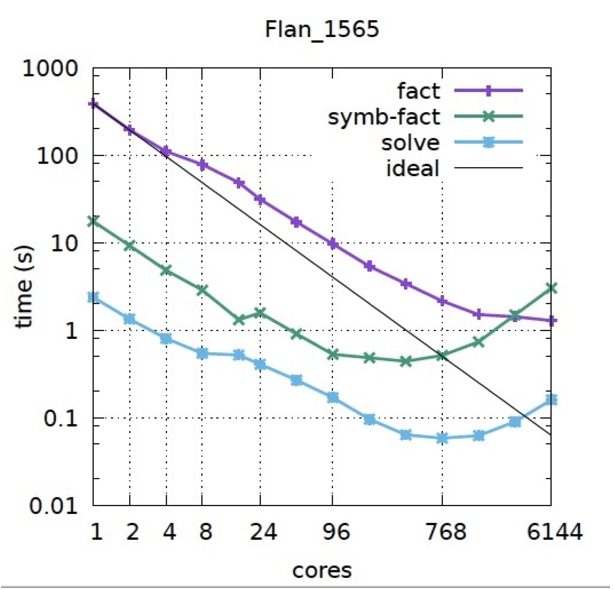
\includegraphics[scale=0.45]{projects/2.3.3-MathLibs/2.3.3.07-STRUMPACK-SuperLU/strumpack-scaling.pdf}
\caption{STRUMPACK scaling of three phases.}
\label{fig:strumpack-scaling}
\end{minipage}
\begin{minipage}[b]{0.48\columnwidth}
\centering
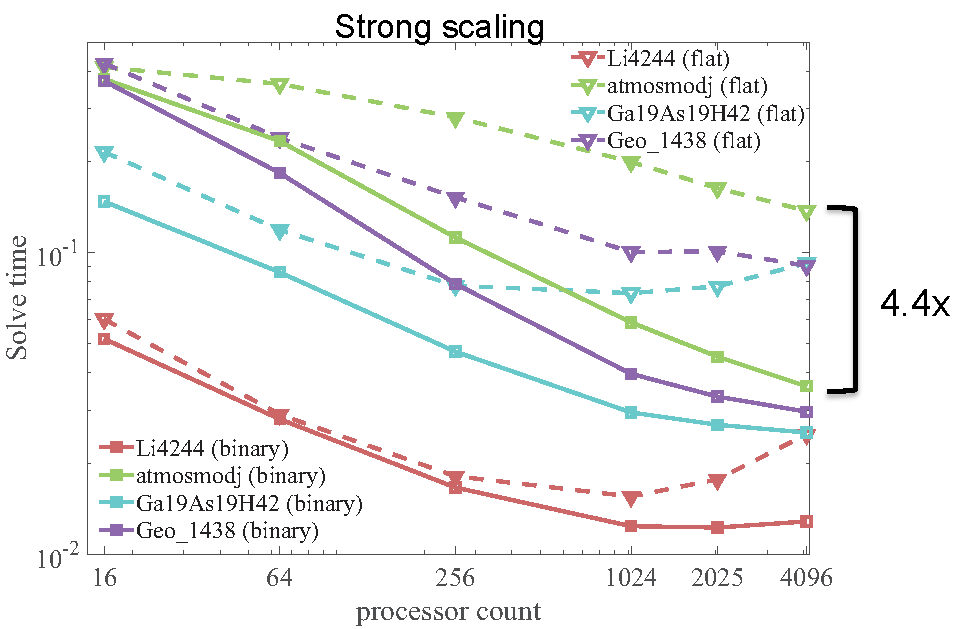
\includegraphics[scale=0.45]{projects/2.3.3-MathLibs/2.3.3.07-STRUMPACK-SuperLU/superlu-trisolve-scaling}
\caption{SuperLU triangular solve scaling with 4 matrices.}
\label{fig:superlu-trisolve}
\end{minipage}
\end{figure}


\paragraph{Next Steps} Our future efforts will focus on the following areas:
%\textit{Describe what you are working on next.}
\begin{itemize}
\item For STRUMPACK, we will improve the performance of the HSS solve
      routine, add OpenMP and reduce communication. We will implement
      the HOLDR low-rank format.
\item For both STRUMPACK and SuperLU, we will build detailed performance
      models and performance specific code optimizations for the ECP
      applications that use our solvers.
\end{itemize}
